\chapter{Experimentos}
\label{cap:capitulo7}

\begin{flushright}
\begin{minipage}[]{10cm}
\emph{Toda la vida es un experimento. Cuantos más experimentos hagas, mejor}\\
\end{minipage}\\

Ralph Waldo Emerson\\
\end{flushright}

\vspace{1cm}

\setcounter{footnote}{132} % Establecer la numeración de la siguiente nota al pie

En este capítulo se tratarán los diferentes experimentos llevados a cabo para la realización de este proyecto y que han permitido conseguir y demostrar la consecución del objetivo y subobjetivos definidos en la Seccción \ref{sec:descripcion}.

\section{Impresión 3D}
\label{sec:expimpresion3d}
Aparte de la solución proporcionada en la Sección \ref{sec:impresionmontaje}, se probaron previamente distintas opciones de diseño y de impresión 3D hasta encontrar la mejor opción.

Primero se optó por diseñar la estructura como una pieza única para facilitar el trabajo de ensamblaje para los usuarios, sin embargo el resultado final no fue el esperado (Figura \ref{fig:imfallida}). 

\begin{figure}[ht!]
	\centering
	\begin{minipage}{0.45\linewidth}
		\centering
		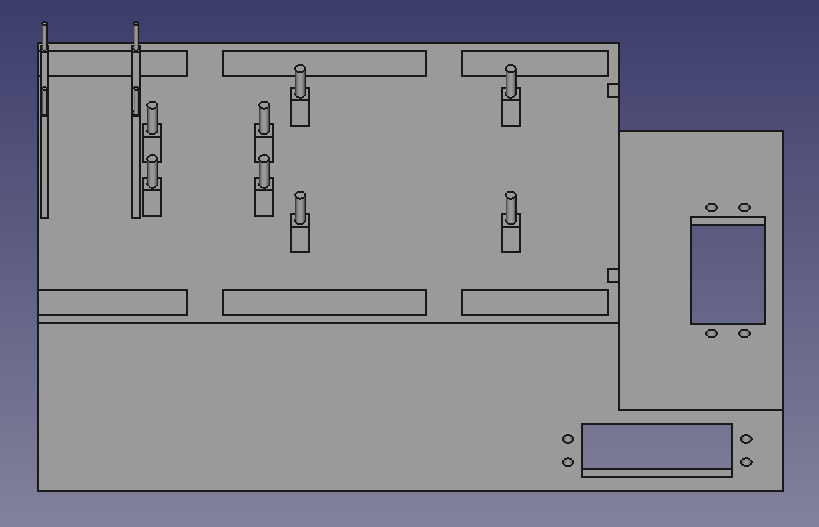
\includegraphics[width=\linewidth]{figs/cap7/impresionfallida1.png}
	\end{minipage}
	\hspace{1cm}
	\begin{minipage}{0.40\linewidth}
		\centering
		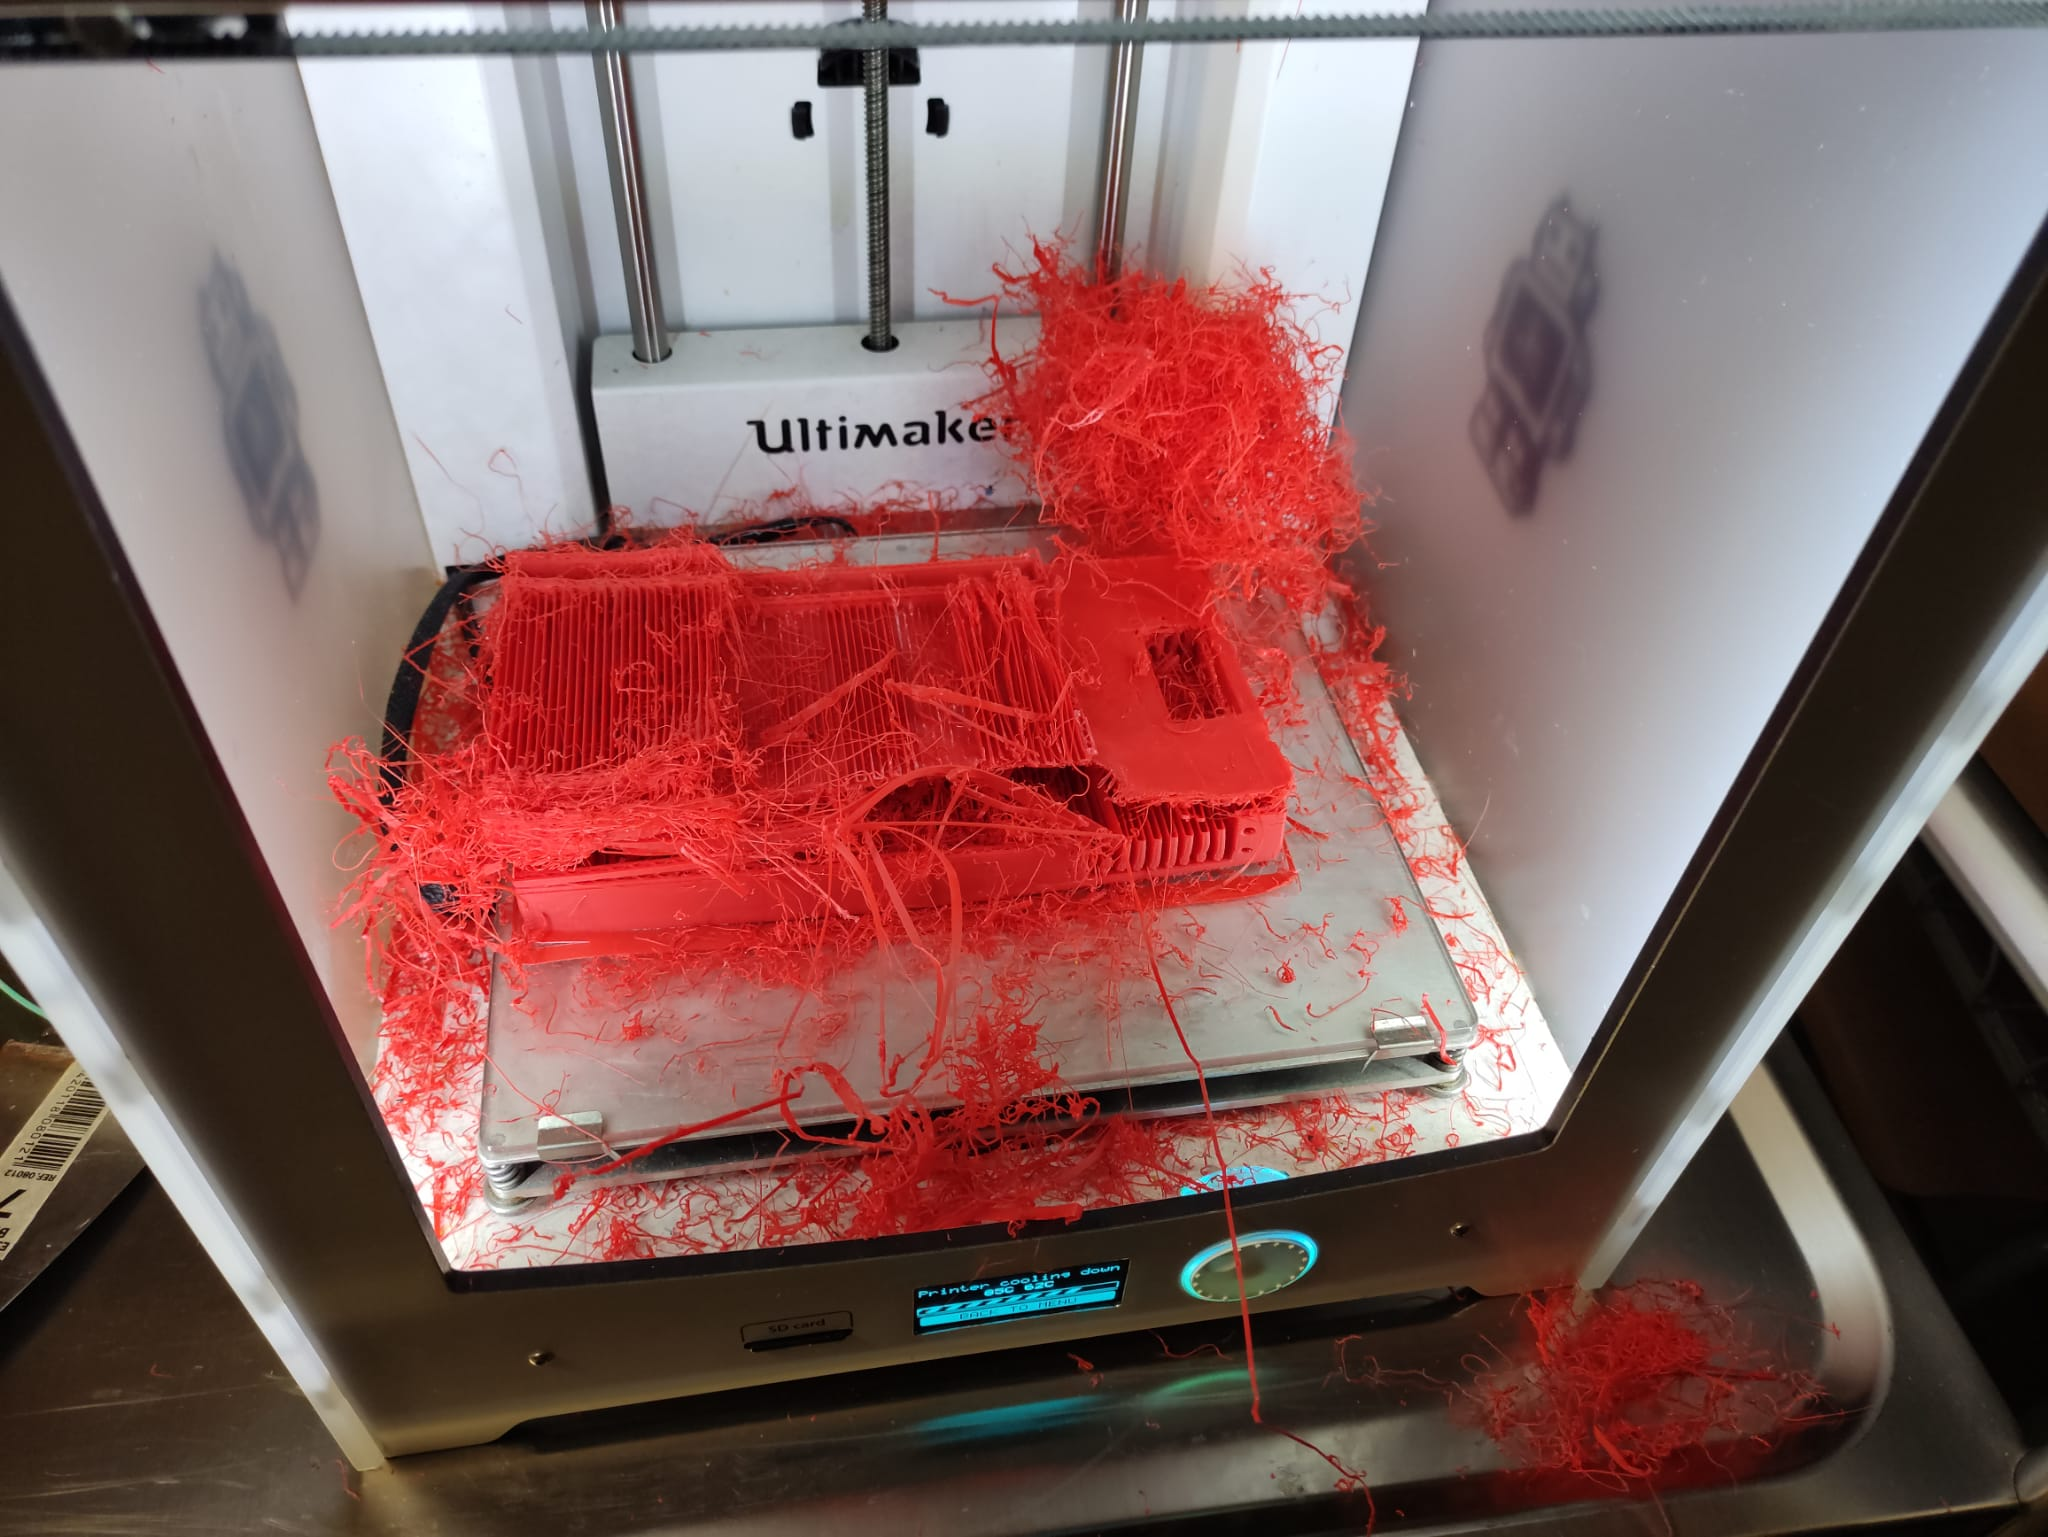
\includegraphics[width=\linewidth]{figs/cap7/piezav1error.jpeg}
	\end{minipage}
	\caption{Versiones previas de impresión}
	\label{fig:imfallida}
\end{figure}


Después de eso, se tuvo que cambiar el enfoque y se decidió dividirlo en diferentes piezas para intentar solucionar el problema, como se comentó en la Sección \ref{sec:diseñocad}. En ese momento se estaba usando otra impresora distinta a la definida en la Sección \ref{sec:impresionmontaje}, llamada Ultimaker Cura 2+\footnote{\url{https://ultimaker.com/3d-printers/s-series/ultimaker-2-connect/}}y se empleó ABS en vez de PLA; por lo tanto, los parámetros de impresión fueron distintos (Cuadro \ref{cuadro:cimpresion2}) pero se producía \textit{warping}. Para conocer más acerca de distintas pruebas, puedes consultarlas en la WIKI\footnote{\url{https://github.com/RoboticsURJC/tfg-jlopez/wiki/HARDWARE\#impresi\%C3\%B3n-3d}}.

\begin{table}[H]
	\begin{center}
		\begin{tabular}{|c|c|}
			\hline
			Características & Parámetros\\
			\hline
			 Densidad & 1.04 g/cm³\\
			\hline
			Diámetro & 2.85 mm\\
			\hline
			Temperatura de impresión & 240 ºC\\
			\hline
			Temperatura de la placa & 110 ºC\\
			\hline
			Temperatura en modo de espera & 175 ºC\\
			\hline
			Distancia de retracción & 6.50 mm\\
			\hline
			Velocidad de retracción & 40mm/s\\
			\hline
			Velocidad del ventilador & 10\%\\
			\hline
		\end{tabular}
		\caption{Características usadas en impresiones previas}
		\label{cuadro:cimpresion2}
	\end{center}
\end{table}

\section{Ruedas}
\label{sec:expruedas}
Como se comentó en la Sección \ref{subsec:ruedas}, en este proyecto se han usado 2 tipos de ruedas que gracias a las distintas pruebas realizadas, se ha podido definir las características de cada una de ellas. 

En el primer video\footnote{\url{}} (Figura \ref{fig:pruebaruedas} izquierda) se puede ver a PiBotJ usando las ruedas negras y teniendo dificultades en superficies con irregularidades. Por otro lado, en el segundo video\footnote{\url{}} (Figura \ref{fig:pruebaruedas} derecha) se puede ver a PiBotJ usando las ruedas azules genéricas y superando con mayor facilidad las dificultades que con las ruedas del kit \textit{ActivityBot}.

%% Incluir 2 vídeos y las dos fotos (capturas del video)

%\begin{figure}[ht!]
%	\centering
%	\begin{minipage}{0.4\linewidth}
%		\centering
%		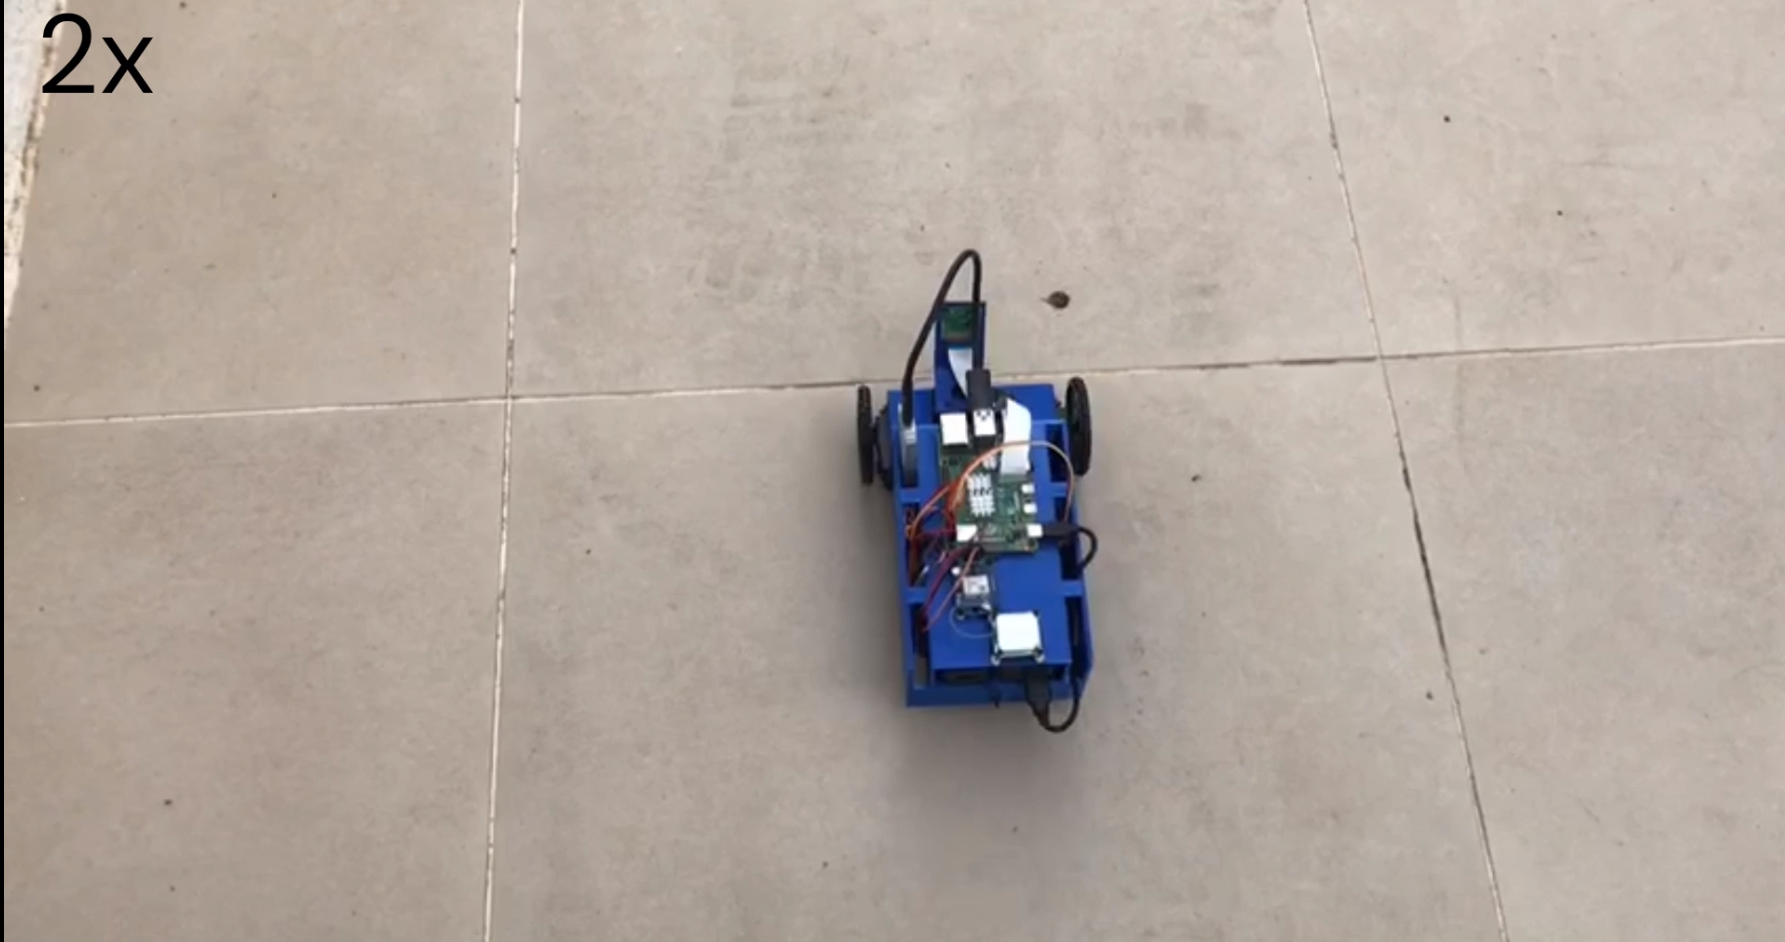
\includegraphics[width=\linewidth]{figs/cap7/pruebanegra.png}
%	\end{minipage}
%	\hspace{1cm}
%	\begin{minipage}{0.40\linewidth}
%		\centering
%		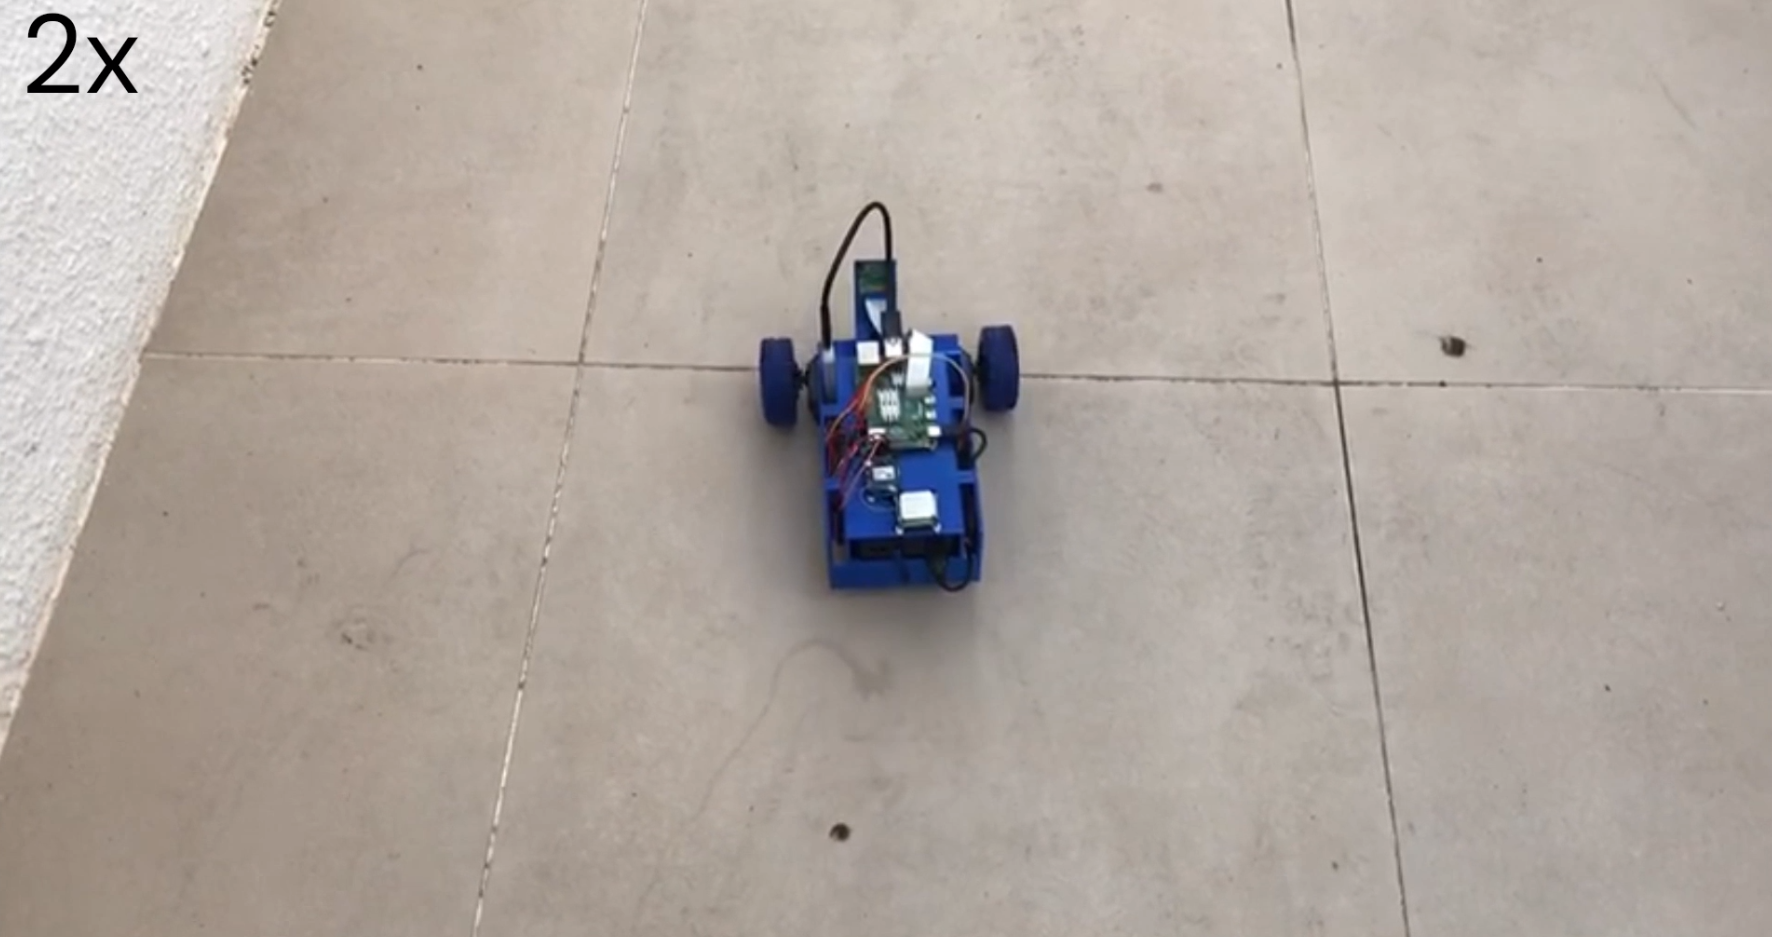
\includegraphics[width=\linewidth]{figs/cap7/pruebaazul.png}
%	\end{minipage}
%	\caption{Versiones previas de impresión}
%	\label{fig:pruebaruedas}
%\end{figure}


\section{Detección de baches}
\label{sec:expaa}

Para conseguir el modelo de entrenamiento de red neuronal creado con YOLOv8, con formato .pb, que se explicó en la Sección \ref{subsec:softwareiayolo}, se realizaron numerosas pruebas pero finalmente para la etapa de entrenamiento se decidió usar la siguiente configuración (Figura \ref{fig:configaa}). Está completamente recogido y facilitado en el fichero \verb|args.yaml|\footnote{\url{https://github.com/RoboticsURJC/tfg-jlopez/blob/main/code/ros2/src/pibotj_rr/custom_model_lite/args.yaml}}.

%\begin{figure} [h!]
%	\begin{center}
%		\includegraphics[width=8cm]{figs/cap7/parametros.png}
%	\end{center}
%	\caption{Parte de la configuración usada para el entrenamiento}
%	\label{fig:configaa}
%\end{figure}\

%% Descripción de la imagen 

Una vez creado, entrenado y convertido el modelo en el formato .tflite, formato compatible con Google Coral, se crearon distintas versiones que se describen a continuación.  
\begin{itemize}
	\item \verb|detect.tflite|\footnote{\url{https://github.com/RoboticsURJC/tfg-jlopez/blob/main/code/ros2/src/pibotj_rr/custom_model_lite/detect.tflite}}. Esta primera versión se realizó usando un dataset de 75 imágenes pero usa CPU y tiene baja reactividad: tiene una latencia de unos cuatro segundos.
	\item \verb|detect_edgetpu.tflite|\footnote{\url{https://github.com/RoboticsURJC/tfg-jlopez/blob/main/code/ros2/src/pibotj_rr/custom_model_lite/detect_edgetpu.tflite}}. Esta versión usa el dataset de 75 imágenes y se intentó que el modelo usase \ac{TPU} del Google Coral pero no funcionó.
	\item \verb|best_full_integer_quant_edgetpu.tflite|\footnote{\url{https://github.com/RoboticsURJC/tfg-jlopez/blob/main/code/ros2/src/pibotj_rr/custom_model_lite/best_full_integer_quant_edgetpu.tflite}}. Esta versión usa el dataset definido en la Sección \ref{subsec:softwareiayolo}. En esta ocasión sí es capar de usar \acs{TPU} pero el modelo se moría a los pocos segundos de inicializarlo y era debido a que procesaba imágenes demasiado grandes.
	\item \verb|bestv2_full_integer_quant_edgetpu.tflite|\footnote{\url{https://github.com/RoboticsURJC/tfg-jlopez/blob/main/code/ros2/src/pibotj_rr/custom_model_lite/bestv2_full_integer_quant_edgetpu.tflite}}. Esta es la la versión actual usada en el proyecto. A diferencia del ejemplo anterior procesa imágenes de 192x192 y así evitamos que el modelo se muera y funcione perfectamente. La latencia se ha reducido a más de un cuarto de la primera versión y permite el correcto funcionamiento del modelo.	
\end{itemize}


En la Sección \ref{subsec:softwareiayolo} también se comenta cómo conseguir que los valores obtenidos sean estables usando \acs{EMA} y a continuación se puede ver una gráfica que demuestra su correcta aplicación (Figura \ref{fig:diagramaema}).

%\begin{figure} [h!]
%	\begin{center}
	%		\includegraphics[width=8cm]{figs/cap7/parametros.png}
	%	\end{center}
%	\caption{Parte de la configuración usada para el entrenamiento}
%	\label{fig:diagramaema}
%\end{figure}\

%% compara los valores de ema con la realidad y estudiar la gráfica.

\subsection{Obtención del contorno y coordenadas del bache}
\label{subsec:expcontorno}

Para la obtención de las coordenadas del bache detectado, se probaron distintas opciones. La primera de ellas fue tomar la imagen en la que se consideraba que tenía bache y a partir de ella, aplicando un desenfoque gaussiano, convirtiéndola en escala de grises, se aplicó el detector de bordes de Canny, utilizando a ojo 80 como umbral mínimo y 180 como umbral máximo. El problema que tenía esta opción era que el contorno a buscar se aplicaba a toda la imagen y no solo dónde se encontraba el bache, produciendose en ocasiones la detección incorrecta (Figura \ref{fig:contornoerror}).

\begin{figure} [h!]
	\begin{center}
			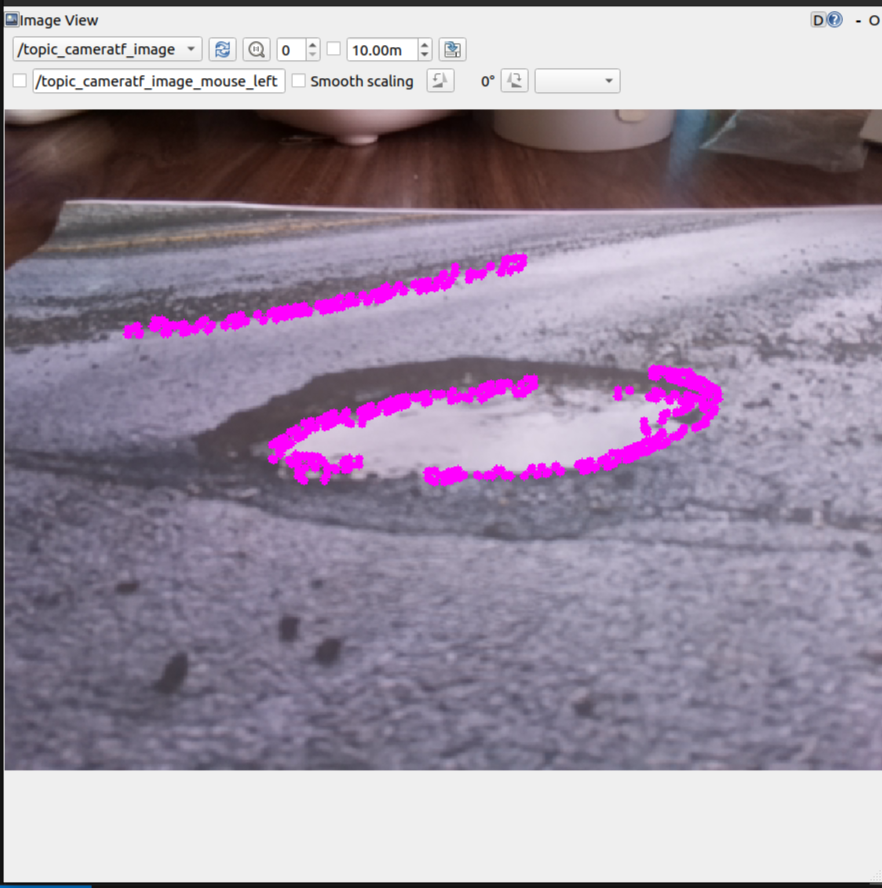
\includegraphics[width=6cm]{figs/cap7/contornoerror.png}
		\end{center}
	\caption{Primera versión en la obtención del contorno del bache}
	\label{fig:contornoerror}
\end{figure}

La segunda y última opción para realizar la detección del contorno, descrita en la Sección \ref{subsec:softwareiayolo} y se puede ver gracias al Código \ref{cod:contorno}. Siendo el valor de 0,6 en el paso de binarizar la máscara, el elegido para decidir si hay bache o no en la imagen. El resultado final se muestra en la Figura \ref{fig:contornobien}.

\begin{code}[h]
	\begin{lstlisting}[language=Python]
		def extract_contour_pixels(self, pothole_mask, resized_frame):
			# Escalar para que aparezca en el tamano correcto
			scale_factor = 192 / 48
			# Binarizar la mascara del bache
			_, binary_mask = cv2.threshold(pothole_mask, 0.6, 1, cv2.THRESH_BINARY)
		
			# Encontrar los contornos del bache
			contours, _ = cv2.findContours(binary_mask.astype(np.uint8), cv2.RETR_EXTERNAL, cv2.CHAIN_APPROX_SIMPLE)
	\end{lstlisting}
	\caption[Cómo obtener el contorno del bache]{Cómo obtener el contorno del bache}
	\label{cod:contorno}
\end{code}

 
 \begin{figure} [h!]
 	\begin{center}
 		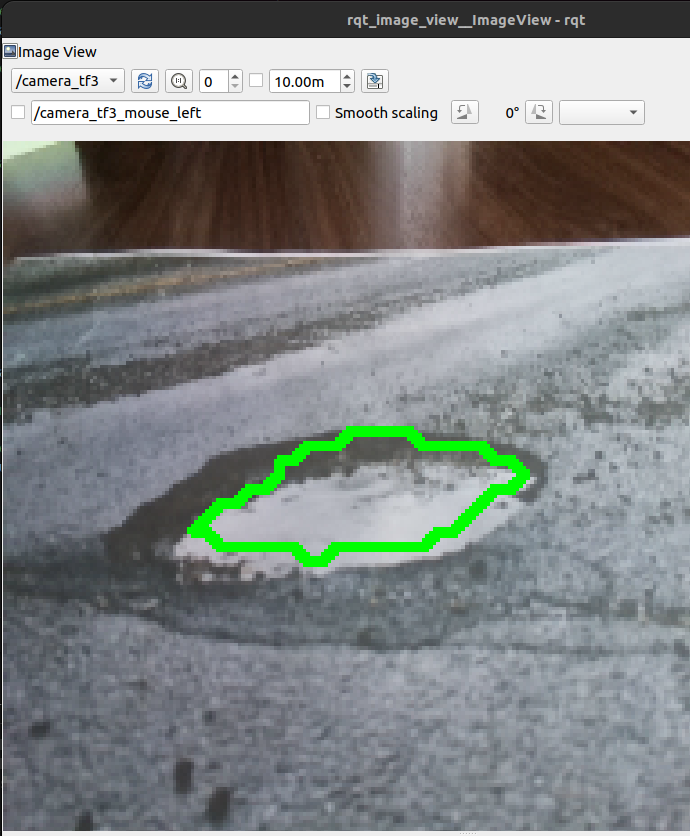
\includegraphics[width=6cm]{figs/cap6/contornobache1.png}
 	\end{center}
 	\caption{Versión final en la obtención del contorno del bache}
 	\label{fig:contornobien}
 \end{figure}


\section{Modelo pinhole}
\label{sec:expmodelopinhole}

Los pasos seguidos para la aplicación del modelo pinhole para la cámara están definidos en la Sección \ref{subsec:softwarehsuelo} pero antes de decidir si el modelo pinhole era adecuado para el proyecto, se realizaron una serie de experimentos. Para la realización de los mismos, se ha usado una cartulina de tamaño A3 pintada de cuadrados de 1x1 cm (Figura \ref{fig:cartulinablanca}) para asegurarnos que las medidas obtenidas eran lo más exactas posibles. El experimento se completa con un círculo recortado de color rosa que será detectado por un filtro de imagen y el algoritmo devolverá la posición del círculo en la vida real. Un ejemplo completo aparece en este video\footnote{\url{}} (Figura \ref{fig:exppinhole}).

\begin{figure} [h!]
	\begin{center}
			
\includegraphics[width=8cm]{figs/cap7/cartulinablanca.jpeg}
		\end{center}
	\caption{Cartulina blanca para probar el modelo pinhole}
	\label{fig:cartulinablanca}
\end{figure}\

%% Captura del video 

%\begin{figure} [h!]
%	\begin{center}
	%		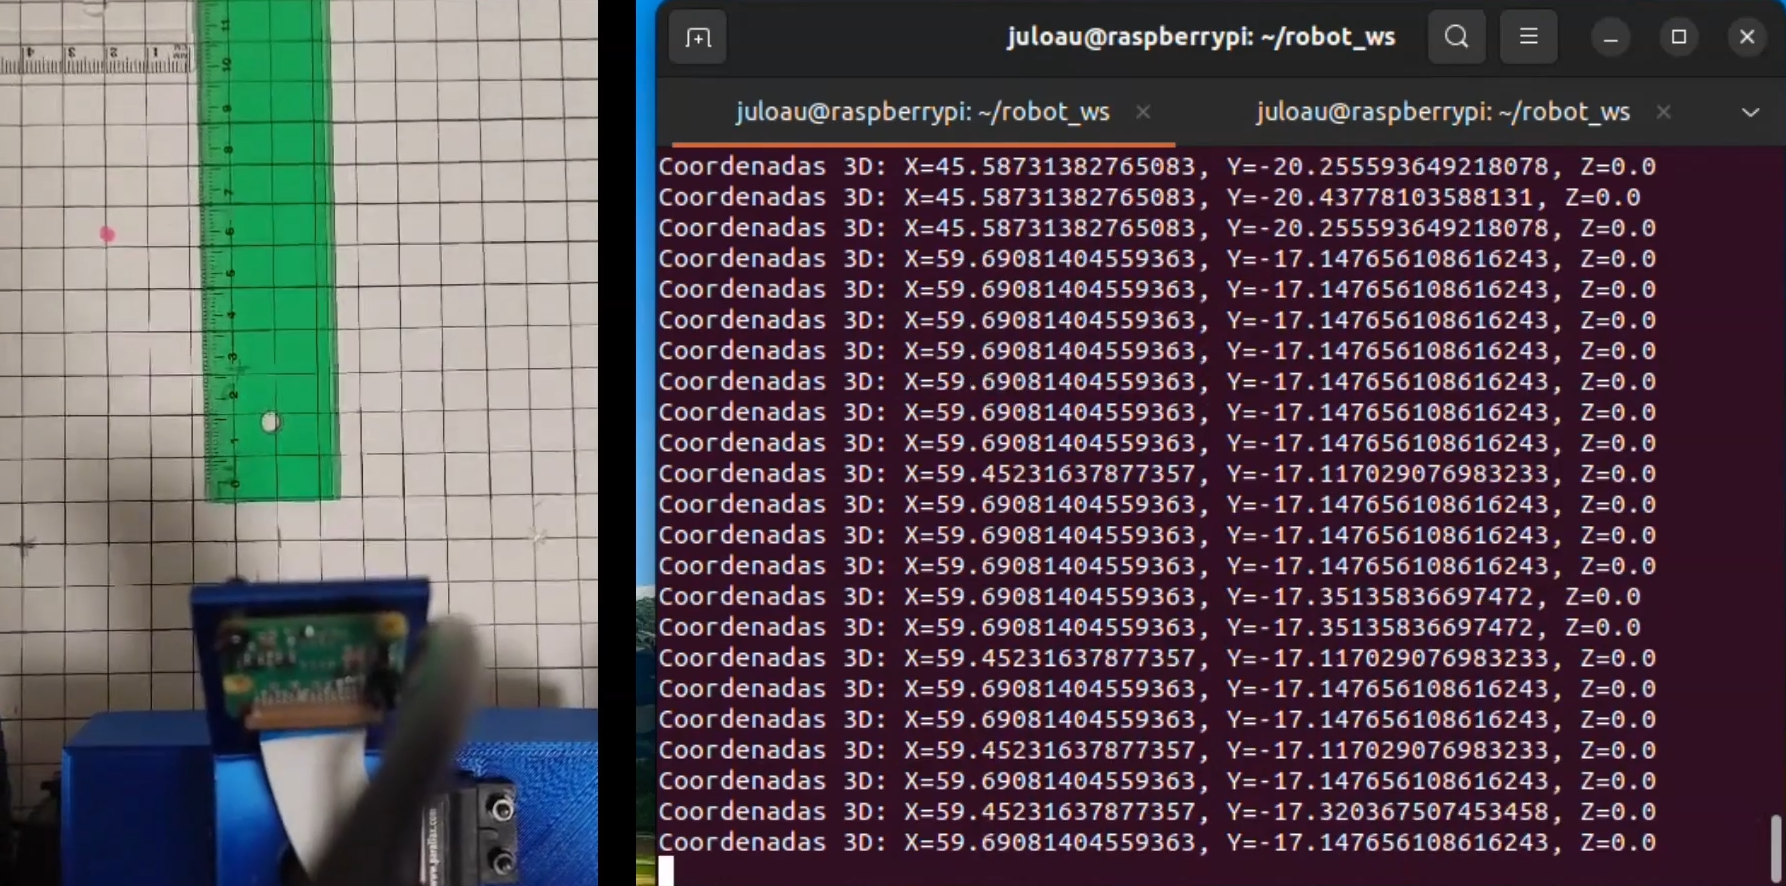
\includegraphics[width=8cm]{figs/cap7/exppinhole.png}
	%	\end{center}
%	\caption{Parte de la configuración usada para el entrenamiento}
%	\label{fig:exppinhole}
%\end{figure}\


\section{Algoritmo de la lazada}
\label{sec:expshoelace}
Al igual que en la Sección \ref{subsec:softwareshoelace} se definió y se ejemplificó de manera teórica el funcionamiento del algoritmo de la lazada, a continuación se va a demostrar su funcionamiento pero en este caso usando un bache. 

%% redactar esta parte: 
%% Incluir imagen del bache con las medidas

%\begin{figure} [h!]
%	\begin{center}
	%		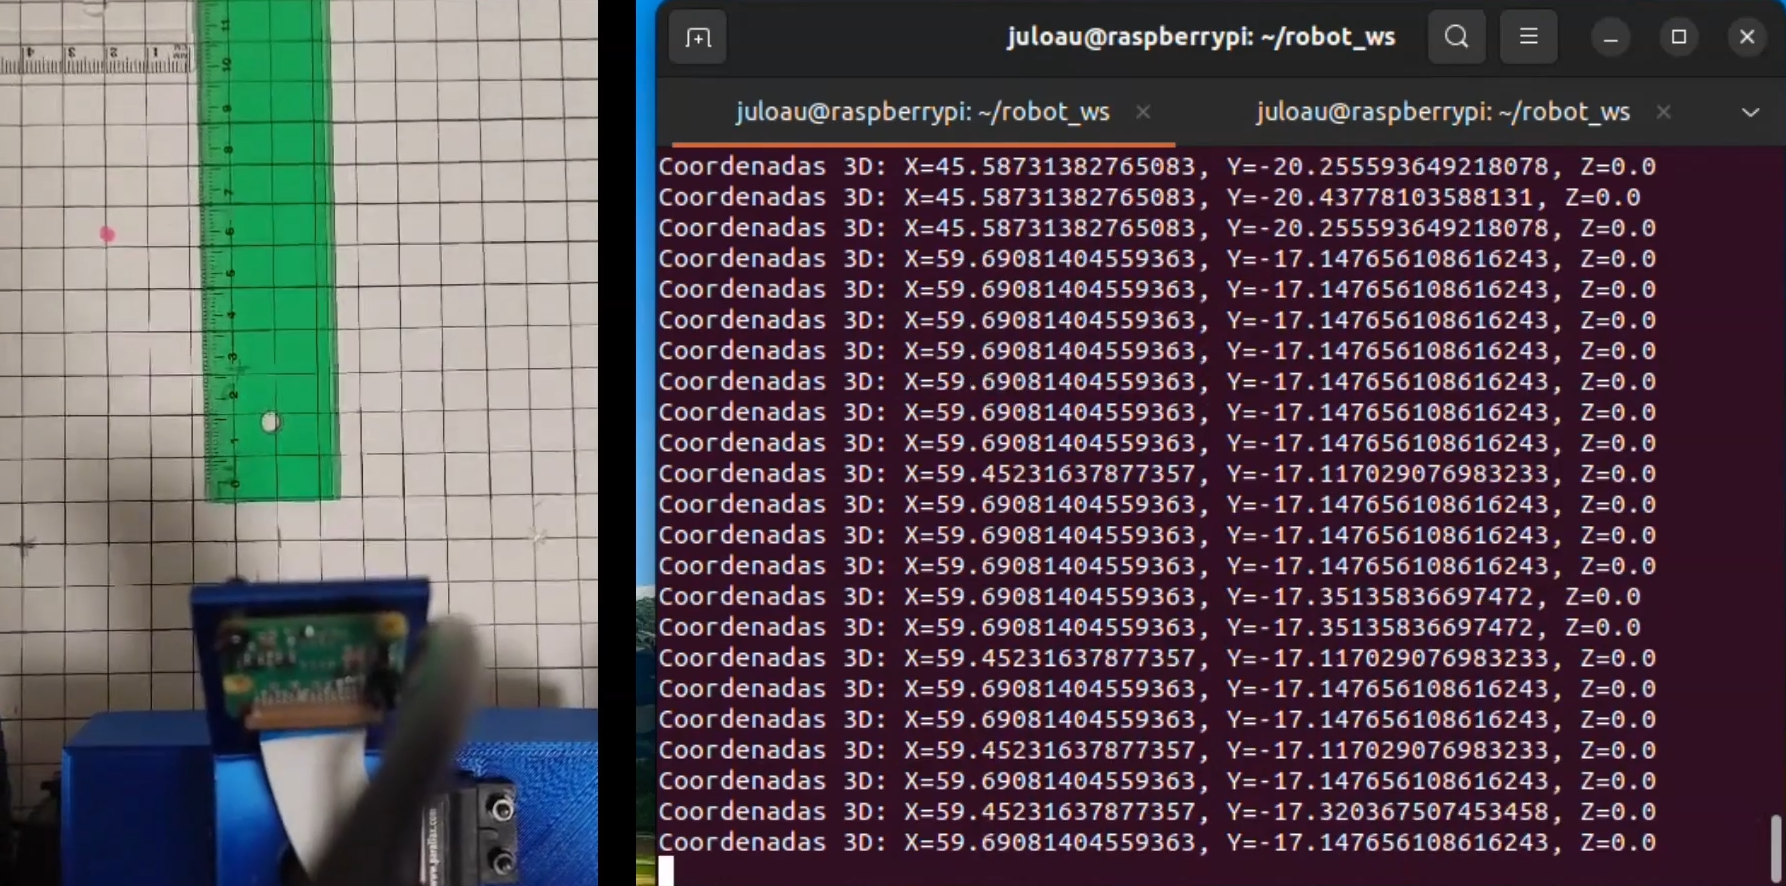
\includegraphics[width=8cm]{figs/cap7/exppinhole.png}
	%	\end{center}
%	\caption{Parte de la configuración usada para el entrenamiento}
%	\label{fig:}
%\end{figure}\


%% incluir el valor del área teórica con una imagen 
%\begin{figure} [h!]
%	\begin{center}
	%		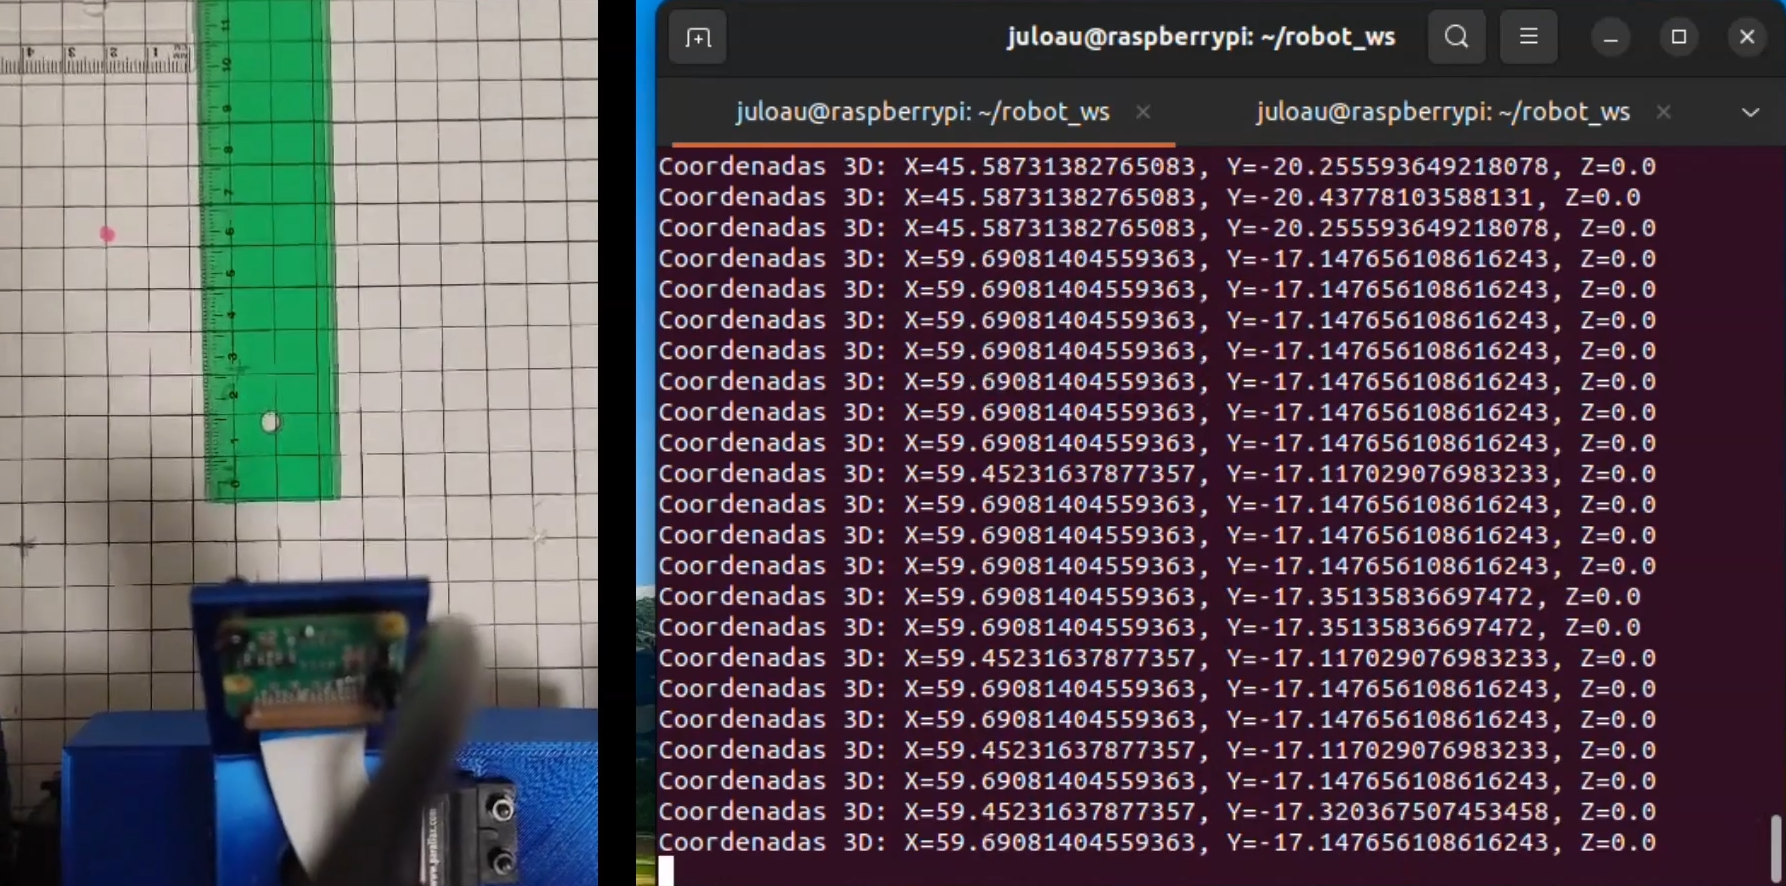
\includegraphics[width=8cm]{figs/cap7/exppinhole.png}
	%	\end{center}
%	\caption{Parte de la configuración usada para el entrenamiento}
%	\label{fig:}
%\end{figure}\


%% incluir una captura del video que muestre el área del bache  usando lazada
%\begin{figure} [h!]
%	\begin{center}
	%		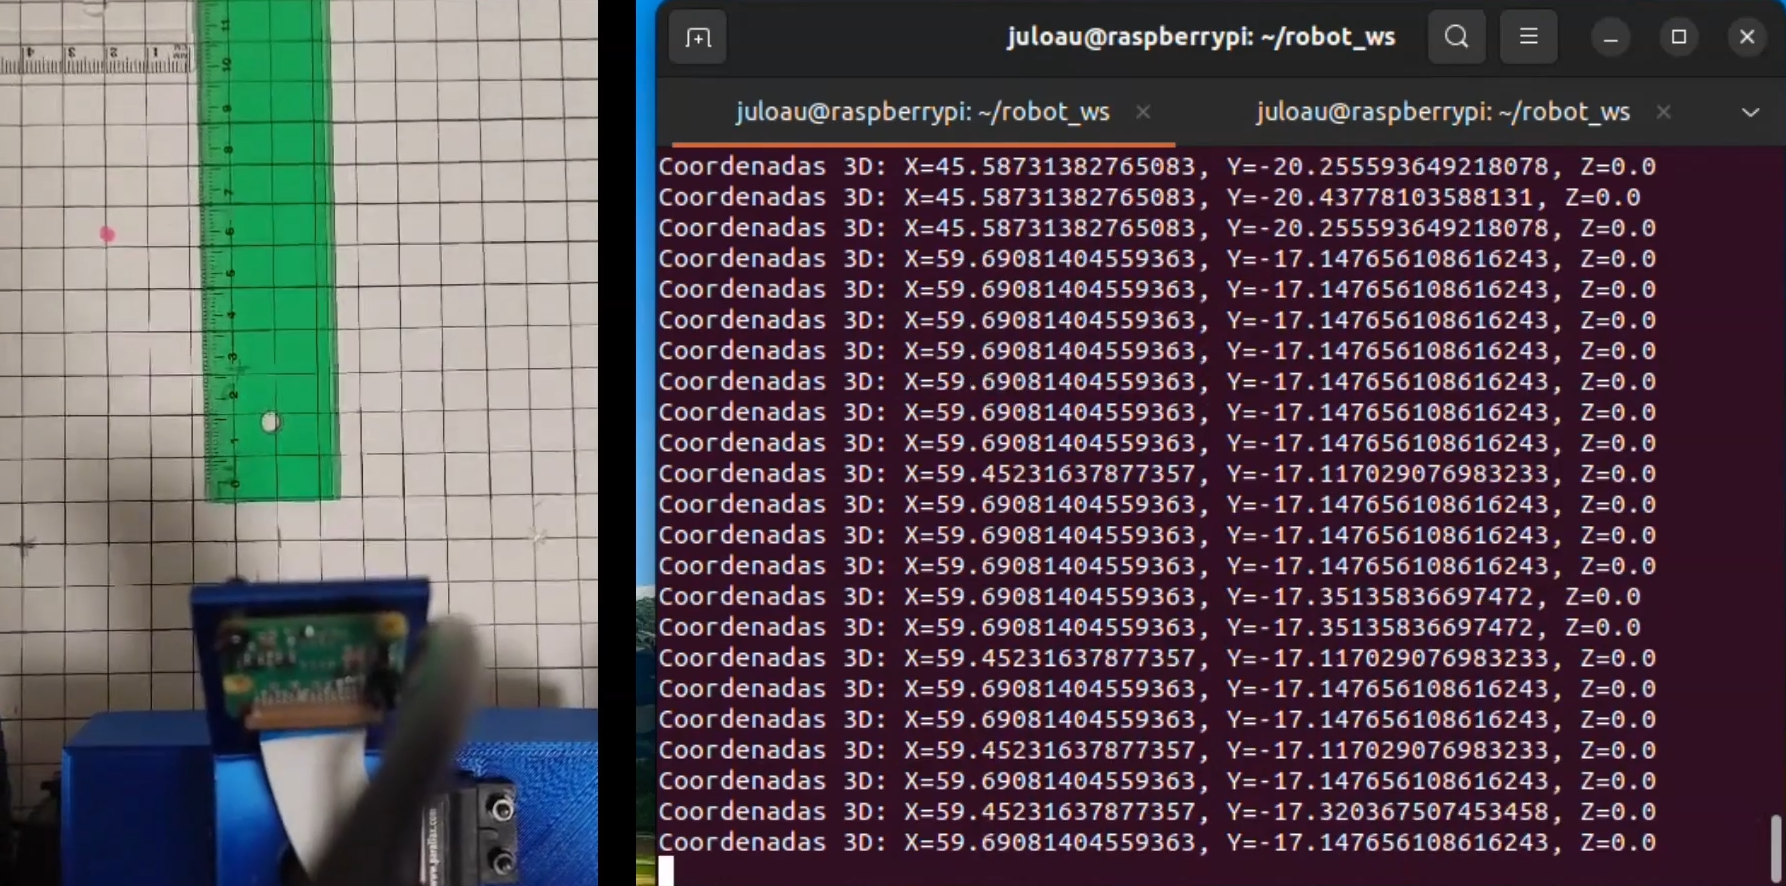
\includegraphics[width=8cm]{figs/cap7/exppinhole.png}
	%	\end{center}
%	\caption{Parte de la configuración usada para el entrenamiento}
%	\label{fig:}
%\end{figure}\



\section{VFF}
\label{sec:expvff}
Para evitar los baches se decidió usar el algoritmo \ac{VFF}, descrito en la Sección \ref{subsec:autonomo}, y para demostrar su funcionamiento, se ha decidido crear un video\footnote{\url{}} que recoge los distintos casos que puede ocurrir (Figura \ref{fig:expvff}).  

% mostrar un video con las distintas fases: no bache, hay bache lejos (no afecta), hay bache cerca (aumenta repulsión) y lo hay cada vez más cerca. 
%\begin{figure} [h!]
%	\begin{center}
	%		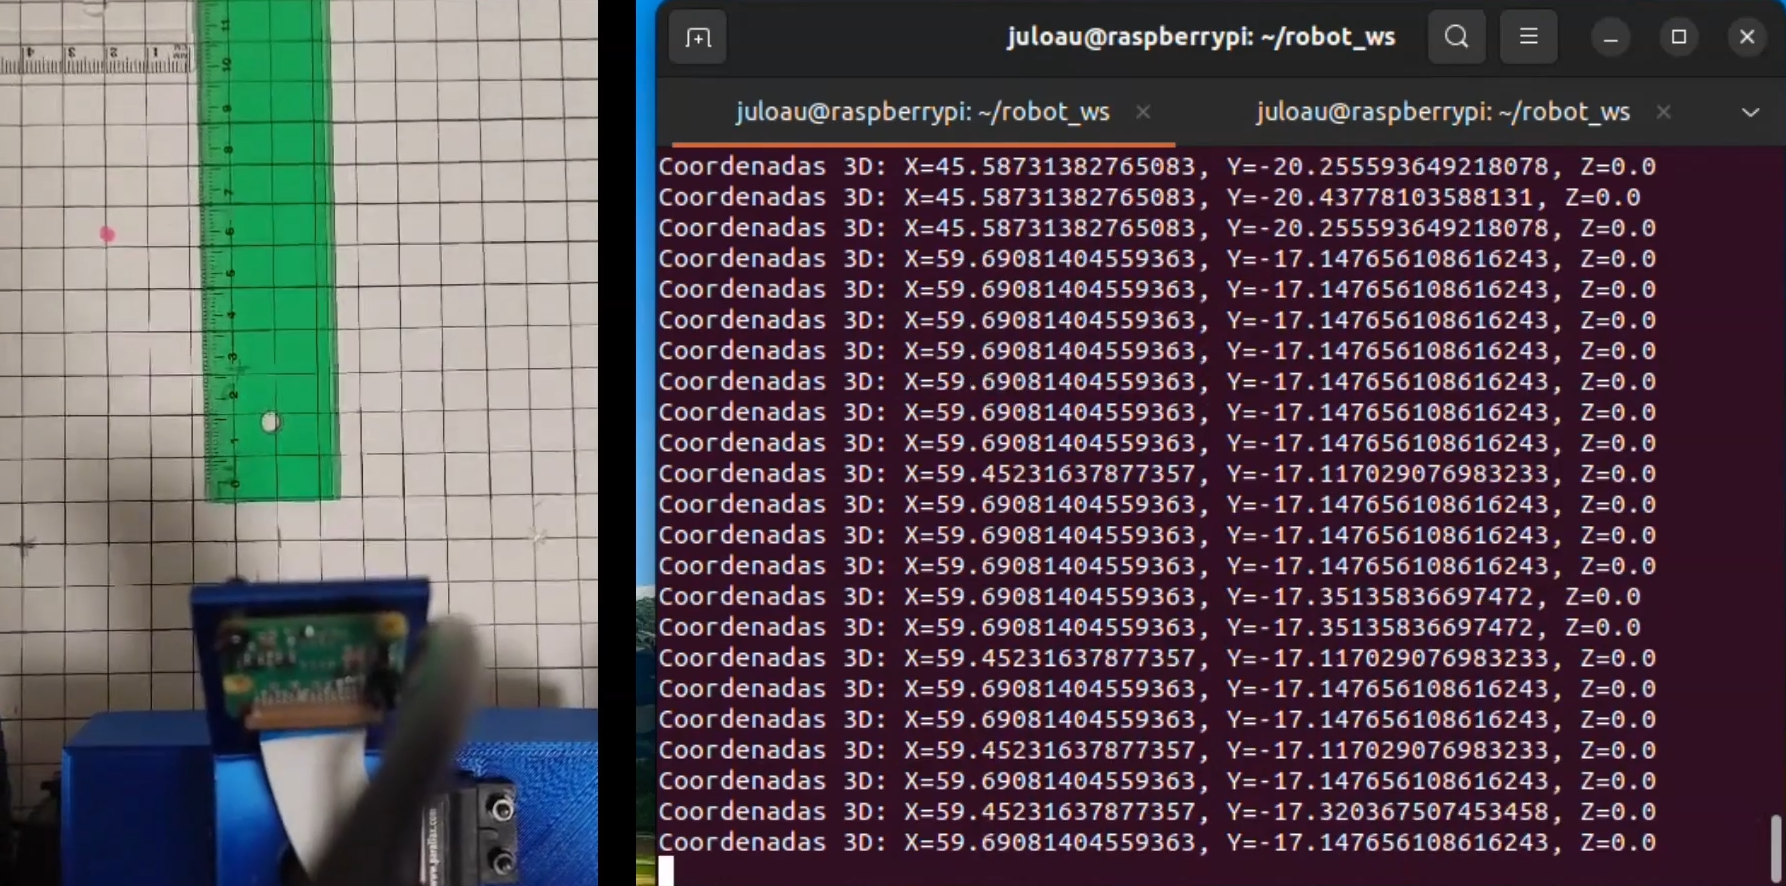
\includegraphics[width=8cm]{figs/cap7/exppinhole.png}
	%	\end{center}
%	\caption{Parte de la configuración usada para el entrenamiento}
%	\label{fig:expvff}
%\end{figure}\

%% Explicar los resultados

%% incluir capturas de pantalla

\section{Ejecución completa de la aplicación}
\label{sec:expcompleto}
A continuación se pueden apreciar los dos ejemplos creados que engloban las posibles opciones que existen de poner en funcionamiento a PiBotJ, que son de forma teleoperada y de forma autónoma. Dentro de cada apartado se podrá apreciar qué comando es necesario lanzar en cada caso, un esquema de cómo funciona cada nodo dentro del \textit{launcher} y capturas de pantalla de cada vídeo.

\subsection{Teleoperado}

Para ejecutar a PiBotJ de forma teleoperada, hay que ejecutar el \textit{launcher}: \verb|ros2 launch pibotj_rr robot_teleop.launch.py|. Dentro del \textit{launcher} se puede distinguir una serie de nodos conectados, como muestra la Figura \ref{fig:nodosteleop}. Una ejecución completa de este ejemplo, se puede apreciar en este video\footnote{\url{}} (Figura \ref{fig:expteleop}). 

%\begin{figure} [h!]
%	\begin{center}
	%		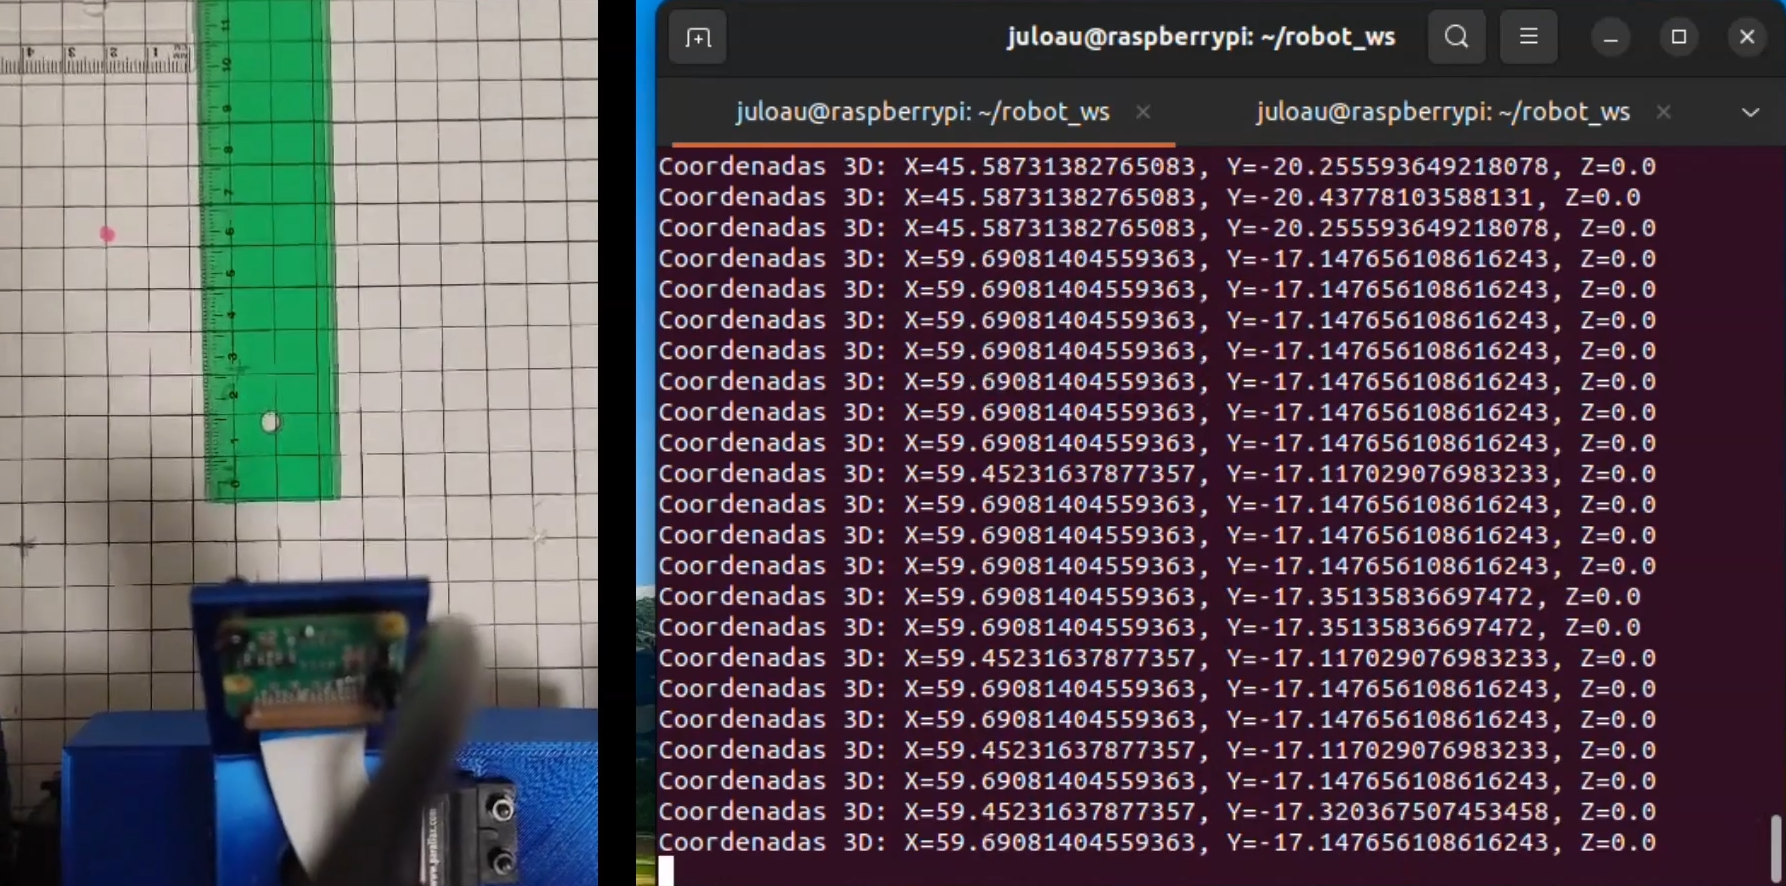
\includegraphics[width=8cm]{figs/cap7/exppinhole.png}
	%	\end{center}
%	\caption{Parte de la configuración usada para el entrenamiento}
%	\label{fig:nodosteleop}
%\end{figure}\
 
%% Capturas de pantalla del video 

%\begin{figure}[ht!]
%	\centering
%	\begin{minipage}{0.4\linewidth}
	%		\centering
	%		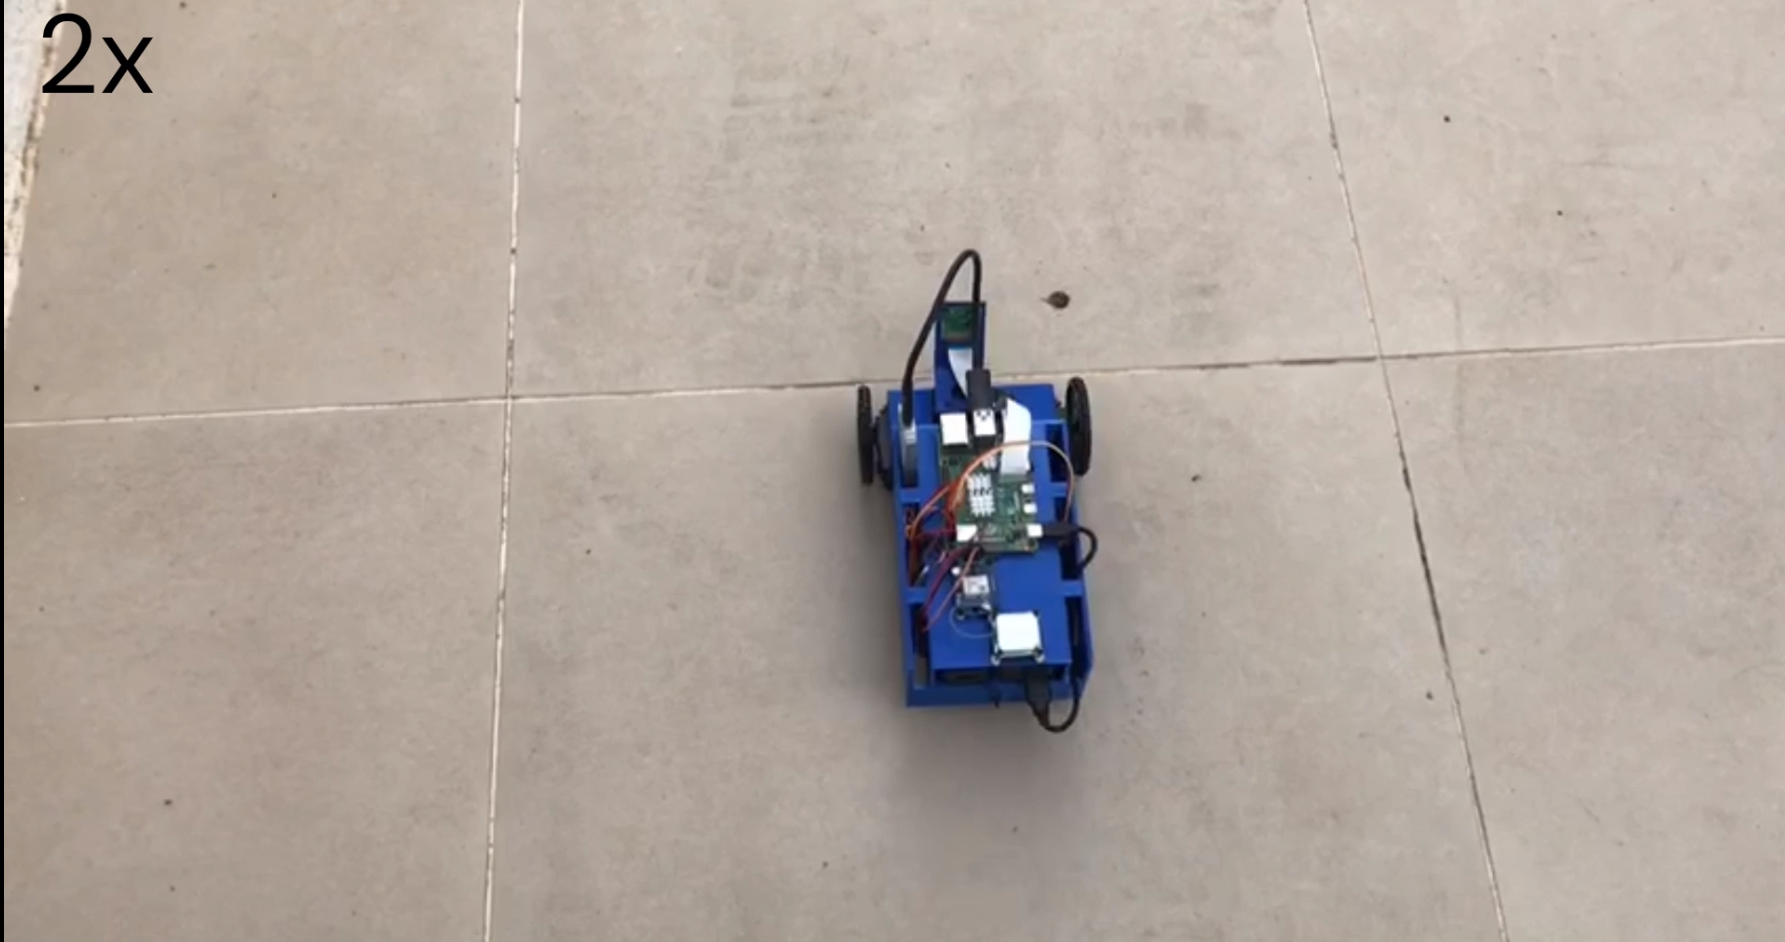
\includegraphics[width=\linewidth]{figs/cap7/pruebanegra.png}
	%	\end{minipage}
%	\hspace{1cm}
%	\begin{minipage}{0.40\linewidth}
	%		\centering
	%		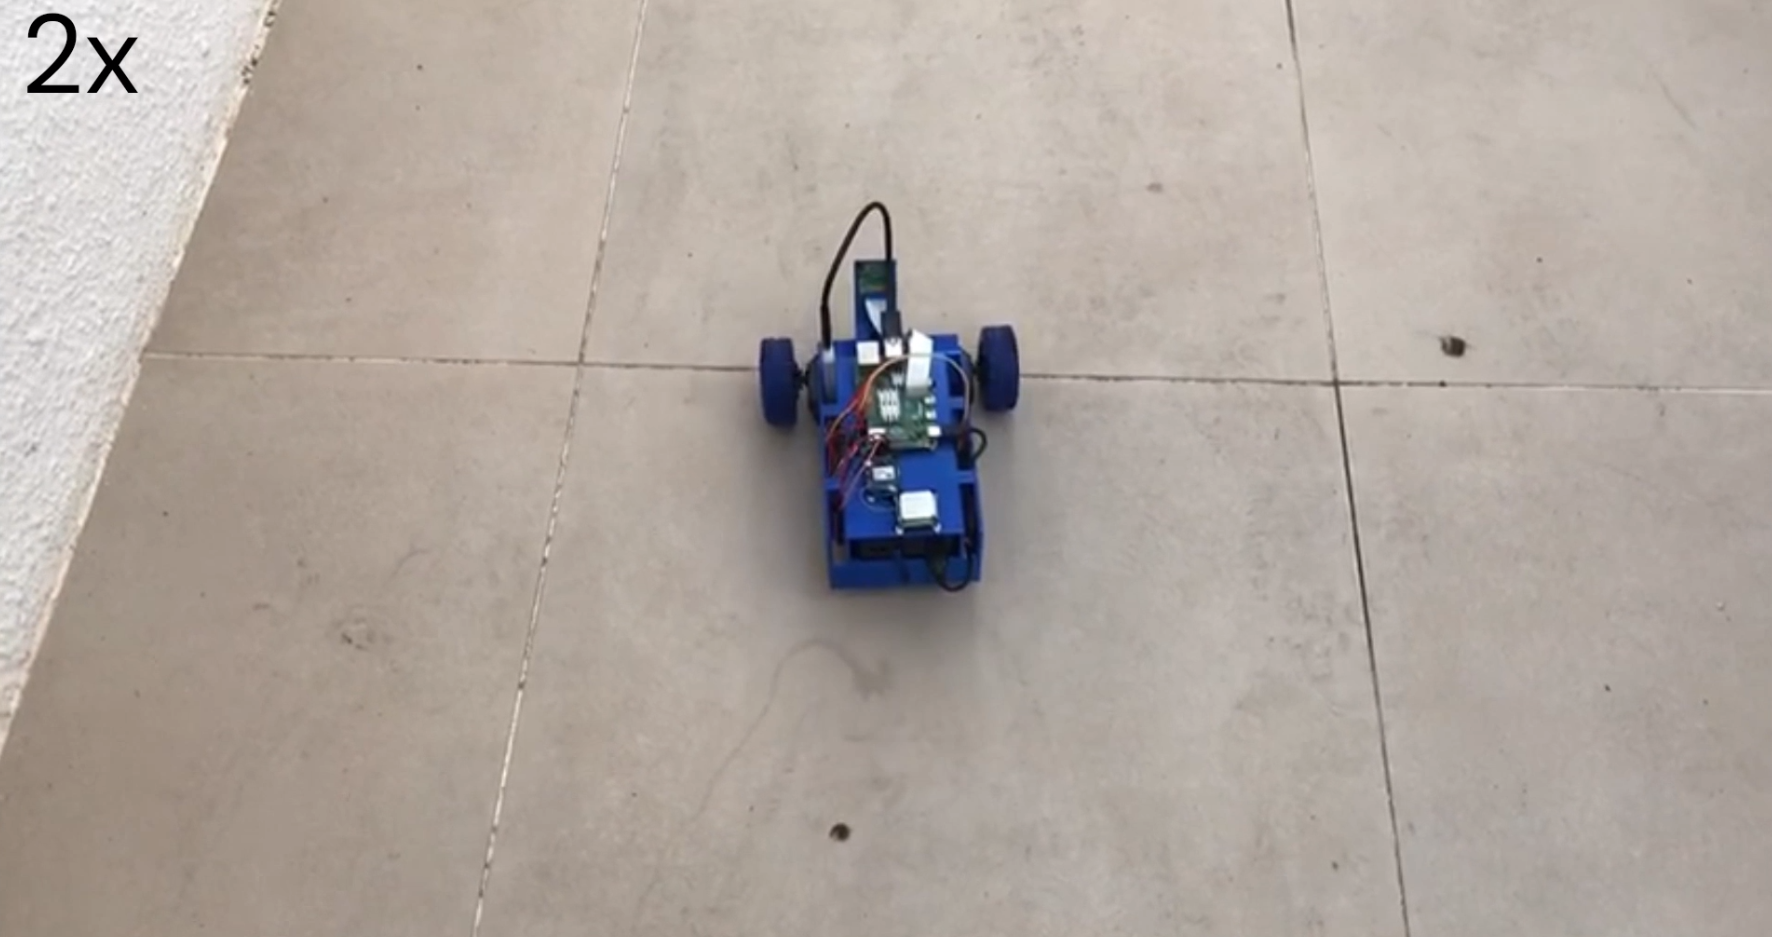
\includegraphics[width=\linewidth]{figs/cap7/pruebaazul.png}
	%	\end{minipage}
%	\caption{Versiones previas de impresión}
%	\label{fig:expteleop}
%\end{figure}


\subsection{Autónomo}

Para ejecutar a PiBotJ de forma autónoma, hay que ejecutar el \textit{launcher}: \verb|ros2 launch pibotj_rr robot_vff.launch.py|. Dentro del \textit{launcher} se puede distinguir una serie de nodos conectados, como muestra la Figura \ref{fig:nodosvff}. Una ejecución completa de este ejemplo, se puede apreciar en este video\footnote{\url{}} (Figura \ref{fig:expvff}). 

%\begin{figure} [h!]
%	\begin{center}
	%		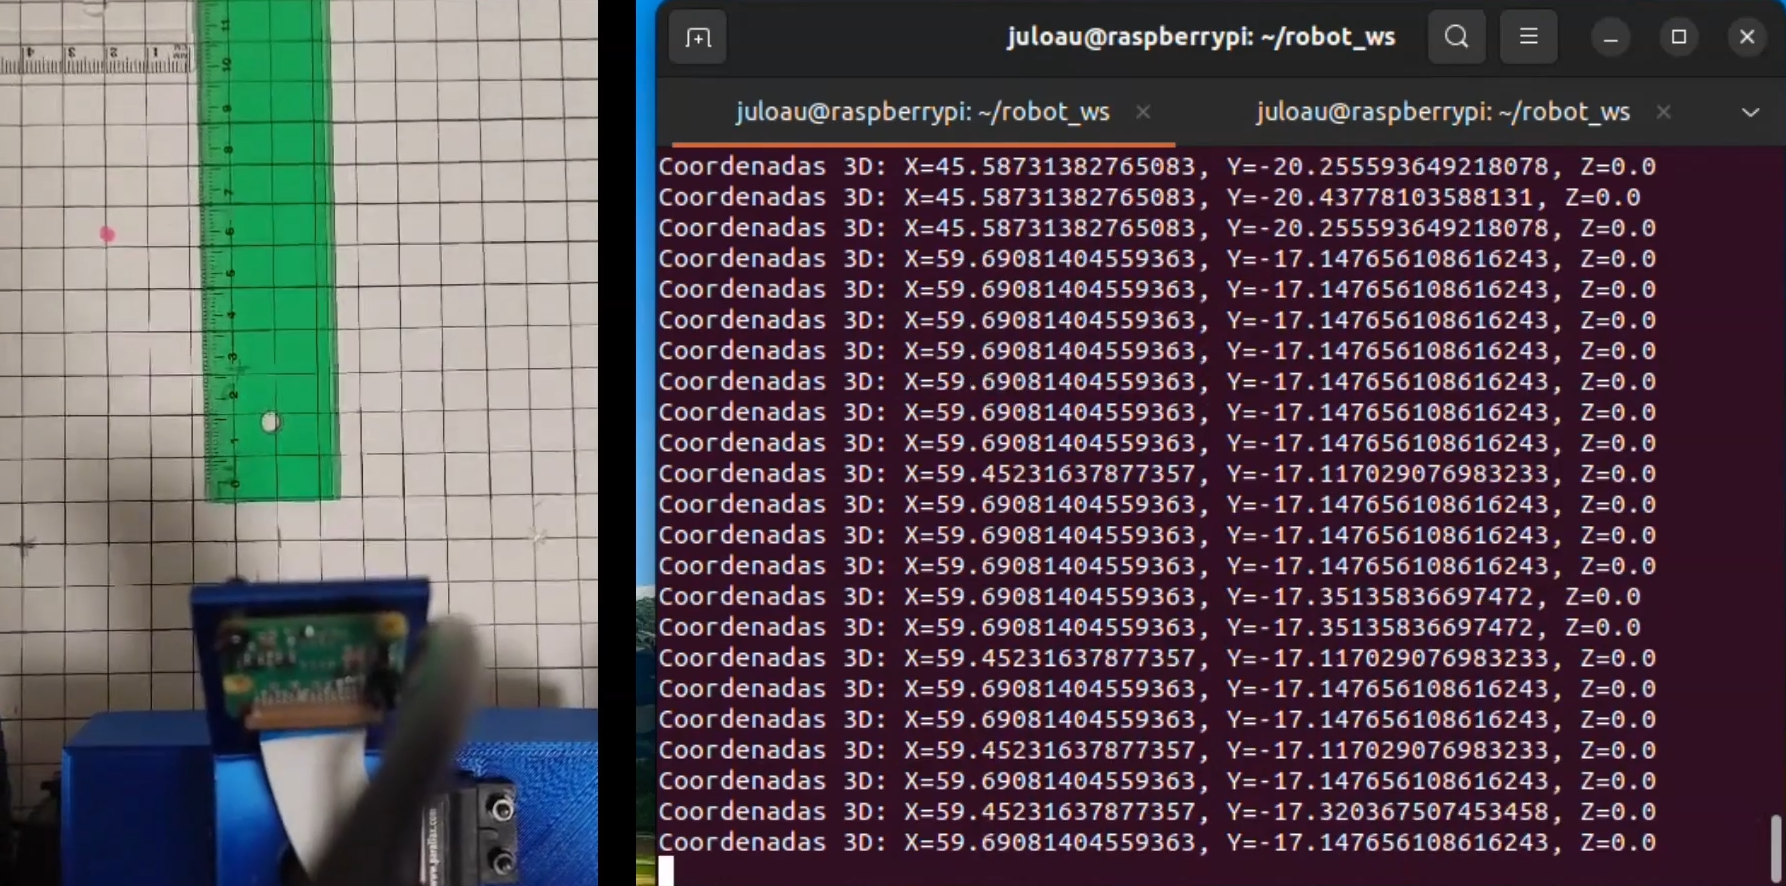
\includegraphics[width=8cm]{figs/cap7/exppinhole.png}
	%	\end{center}
%	\caption{Parte de la configuración usada para el entrenamiento}
%	\label{fig:nodosvff}
%\end{figure}\

%% Capturas de pantalla del video 

%\begin{figure}[ht!]
%	\centering
%	\begin{minipage}{0.4\linewidth}
	%		\centering
	%		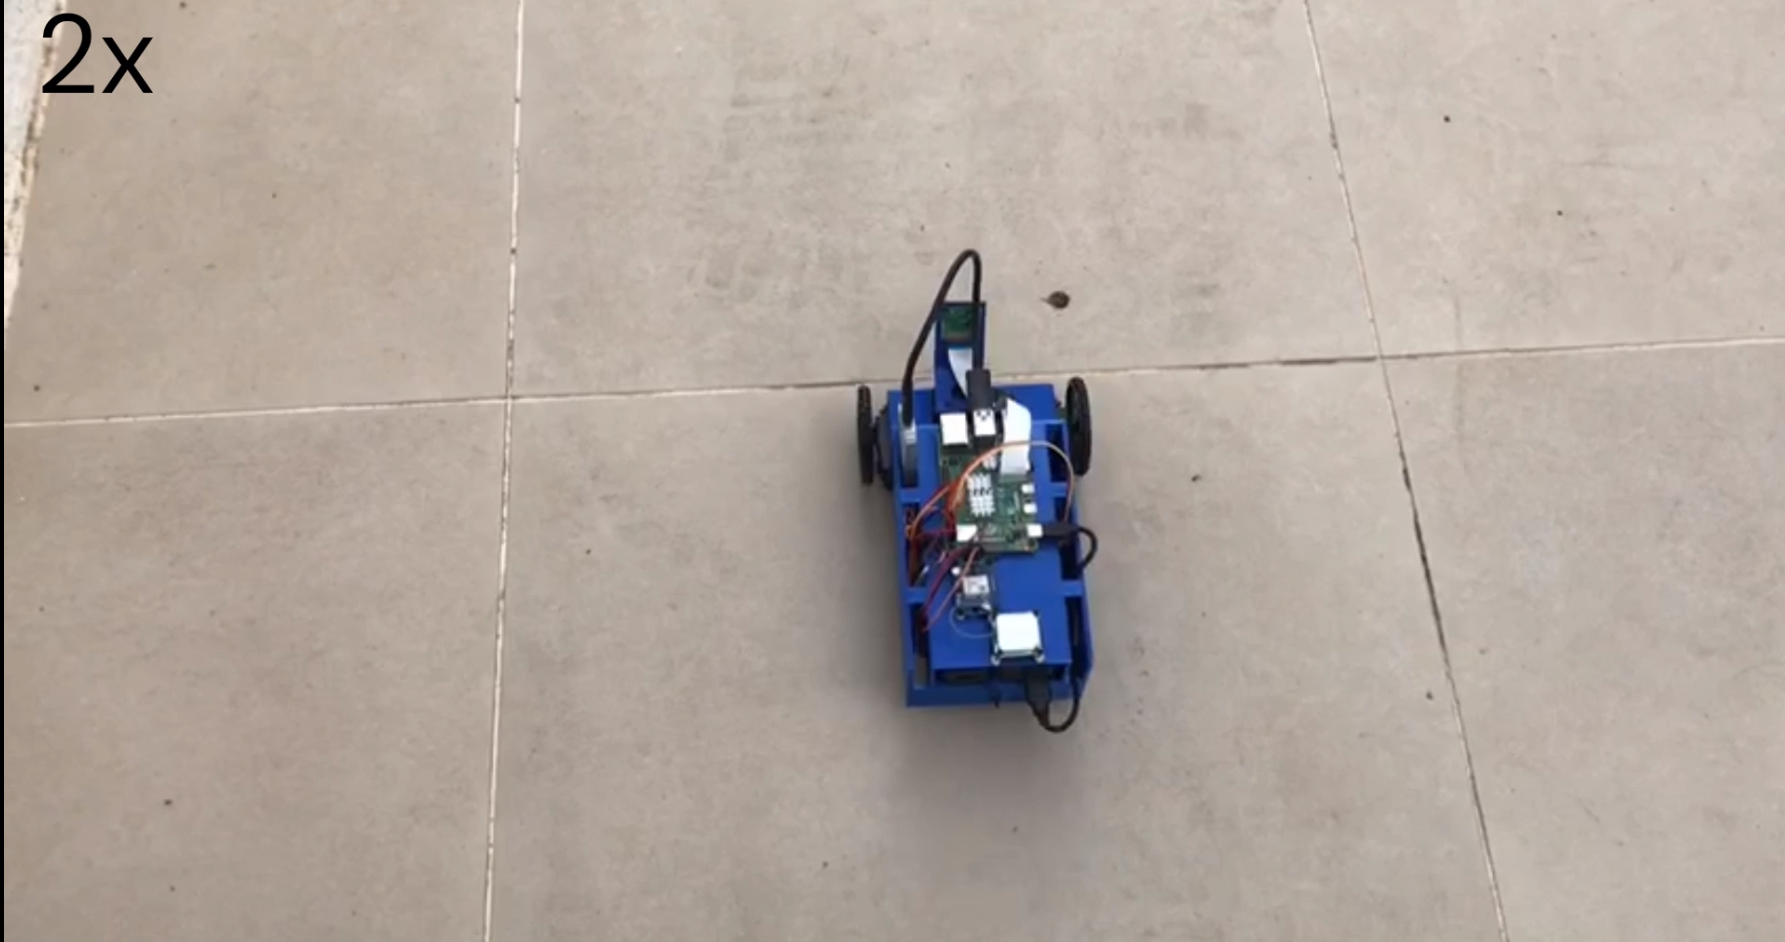
\includegraphics[width=\linewidth]{figs/cap7/pruebanegra.png}
	%	\end{minipage}
%	\hspace{1cm}
%	\begin{minipage}{0.40\linewidth}
	%		\centering
	%		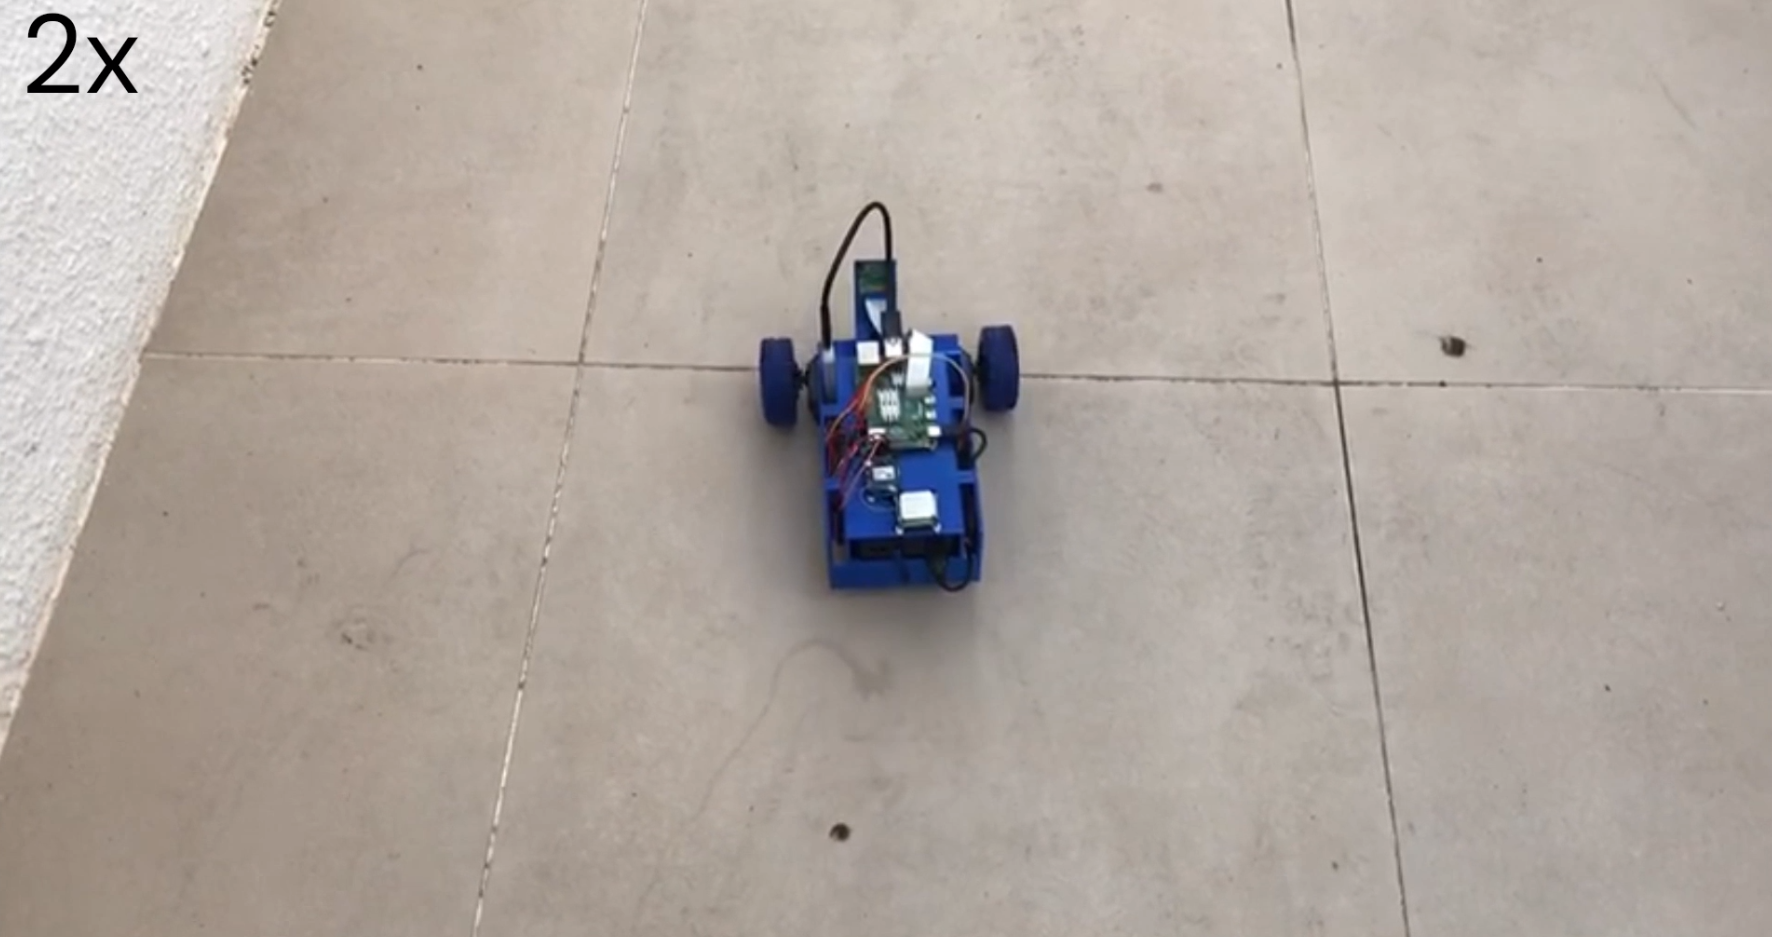
\includegraphics[width=\linewidth]{figs/cap7/pruebaazul.png}
	%	\end{minipage}
%	\caption{Versiones previas de impresión}
%	\label{fig:expvff}
%\end{figure}


\section{Snippets}

Puede resultar interesante, para clarificar la descripción, mostrar fragmentos de código (o \textit{snippets}) ilustrativos. En el Código \ref{cod:codejemplo} vemos un ejemplo escrito en \texttt{C++}.

\begin{code}[h]
	\begin{lstlisting}[language=C++]
		void Memory::hypothesizeParallelograms () {
			for(it1 = this->controller->segmentMemory.begin(); it1++) {
				squareFound = false; it2 = it1; it2++;
				while ((it2 != this->controller->segmentMemory.end()) && (!squareFound)) {
					if (geometry::haveACommonVertex((*it1),(*it2),&square)) {
						dist1 = geometry::distanceBetweenPoints3D ((*it1).start, (*it1).end);
						dist2 = geometry::distanceBetweenPoints3D ((*it2).start, (*it2).end);
					}
					// [...]
				\end{lstlisting}
				\caption[Función para buscar elementos 3D en la imagen]{Función para buscar elementos 3D en la imagen}
				\label{cod:codejemplo}
			\end{code}
			
			En el Código \ref{cod:codejemplo2} vemos un ejemplo escrito en \texttt{Python}.
			
			\begin{code}[h]
				\begin{lstlisting}[language=Python]
					def mostrarValores():
					print (w1.get(), w2.get())
					
					master = Tk()
					w1 = Scale(master, from_=0, to=42)
					w1.pack()
					w2 = Scale(master, from_=0, to=200, orient=HORIZONTAL)
					w2.pack()
					Button(master, text='Show', command=mostrarValores).pack()
					
					mainloop()
				\end{lstlisting}
				\caption[Cómo usar un Slider]{Cómo usar un Slider}
				\label{cod:codejemplo2}
			\end{code}
			
			\section{Verbatim}
			
			Para mencionar identificadores usados en el código ---como nombres de funciones o variables--- en el texto, usa el entorno literal o verbatim \verb|hypothesizeParallelograms()|. También se puede usar este entorno para varias líneas, como se ve a continuación:
			
			\begin{verbatim}
				void Memory::hypothesizeParallelograms () {
					// add your code here
				}
			\end{verbatim}
			
			\section{Ecuaciones}
			
			Si necesitas insertar alguna ecuación, puedes hacerlo. Al igual que las figuras, no te olvides de referenciarlas. A continuación se exponen algunas ecuaciones de ejemplo: Ecuación \ref{ec:ec1} y Ecuación \ref{ec:ec2}.
			
			\begin{myequation}[h]
				\begin{equation}
					H = 1 - \frac{\sum_{i=0}^{N}\frac{(\frac{d_{j_s} + d_{j_e}}{2})}{N}}{M}
					\nonumber
					\label{ec:ec1}
				\end{equation}
				\caption[Ejemplo de ecuación con fracciones]{Ejemplo de ecuación con fracciones}
			\end{myequation} 
			
			\begin{myequation}[h]
				\begin{equation}
					v(entrada)= \left\{
					\begin{array}{lcc}
						0 & \mbox{if} & \epsilon_t < 0.1\\
						K_p\cdot{(T_{t}-T)} & \mbox{if}& 0.1 \leq \epsilon_t < M_t\\
						K_p \cdot M_t & \mbox{if}& M_t < \epsilon_t
					\end{array}
					\right.
					\label{ec:ec2}
				\end{equation}
				\caption[Ejemplo de ecuación con array y letras y símbolos especiales]{Ejemplo de ecuación con array y letras y símbolos especiales}
			\end{myequation}
			
			\section{Tablas o cuadros}
			
			Si necesitas insertar una tabla, hazlo dígnamente usando las propias tablas de \LaTeX, no usando pantallazos e insertándolas como figuras... En el Cuadro \ref{cuadro:ejemplo} vemos un ejemplo.
			
			\begin{table}[H]
				\begin{center}
					\begin{tabular}{|c|c|}
						\hline
						\textbf{Parámetros} & \textbf{Valores} \\
						\hline
						Tipo de sensor & Sony IMX219PQ[7] CMOS 8-Mpx \\
						Tamaño del sensor & 3.674 x 2.760 mm (1/4" format) \\
						Número de pixels & 3280 x 2464 (active pixels) \\
						Tamaño de pixel & 1.12 x 1.12 um \\
						Lente & f=3.04 mm, f/2.0 \\
						Ángulo de visión & 62.2 x 48.8 degrees \\
						Lente SLR equivalente & 29 mm \\
						\hline
					\end{tabular}
					\caption{Parámetros intrínsecos de la cámara}
					\label{cuadro:ejemplo}
				\end{center}
			\end{table}
			
			En los textos puedes poner palabras en \textit{cursiva}, para aquellas expresiones en sentido \textit{figurado}, palabras como \textit{robota}, que está fuera del diccionario castellano, o bien para resaltar palabras de una colección: \textit{(a)} es la primera letra del abecedario, \textit{(b)} es la segunda, etc.\\
			
			Al poner las dos líneas del anterior párrafo, este aparecerá separado del anterior. Si no las pongo, los párrafos aparecerán pegados. Sigue el criterio que consideres más oportuno.
			
			\section{Segunda sección}
			\label{sec:segundaseccion}
			
			No olvides incluir imágenes y referenciarlas, como la Figura \ref{fig:roomba}.
			
			\begin{figure} [h!]
				\begin{center}
					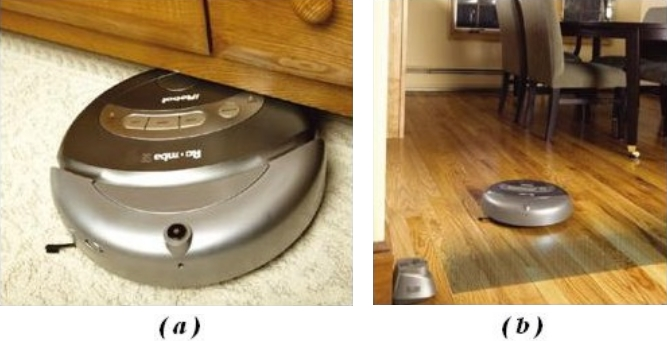
\includegraphics[width=8cm]{figs/roomba}
				\end{center}
				\caption{Robot aspirador Roomba de iRobot.}
				\label{fig:roomba}
			\end{figure}\
			
			Ni tampoco olvides de poner las URLs como notas al pie. Por ejemplo, si hablo de la Robocup\footnote{\url{http://www.robocup.org}}.
			
			\subsection{Números}
			\label{sec:subseccion}
			
			En lugar de tener secciones interminables, como la Sección \ref{sec:robotica}, divídelas en subsecciones.
			
			Para hablar de números, mételos en el entorno \textit{math} de \LaTeX, por ejemplo, $1.5Kg$. También puedes usar el símbolo del Euro como aquí: 1.500\euro.
			
			\subsection{Listas}
			
			Cuando describas una colección, usa \texttt{itemize} para ítems o \texttt{enumerate} para enumerados. Por ejemplo:
			
			\begin{itemize}
				\item \textit{Entorno de simulación.} Hemos usado dos entornos de simulación: uno en 3D y otro en 2D.
				\item \textit{Entornos reales.} Dentro del campus, hemos realizado experimentos en Biblioteca y en el edificio de Gestión.
			\end{itemize}\
			
			\begin{enumerate}
				\item Primer elemento de la colección.
				\item Segundo elemento de la colección.
			\end{enumerate}\
			

